\section{Results}\label{sec:results}

\subsection{Calibration of the paired tests}\label{sec:res-cal}
With no change between tumour and normal, on verification seeds with the final code, the Level~1 test of the $\Hone$ asymmetry rejected at the 0.05 level in \calNormalL\% of \calNormalN{} data sets with normal noise (95\% confidence interval \calNormalLci\%) and in \calOutliersL\% of \calOutliersN{} with outlying specimens (\calOutliersLci\%); Holm's procedure over the gene family rejected at least one gene in \calNormalG\% and \calOutliersG\% (Table~\ref{tab:calibration}). The development runs, with the standardised change, gave \calDevNormalL\%, \calTthreeL\% and \calSkewedL\% for normal, heavy-tailed $t_3$ and skewed noise, and \calDevNormalG\%, \calTthreeG\% and \calSkewedG\% for the gene family. None of the ten runs showed excess rejection at the pre-specified gate. The Level~1 $p$-values were close to uniform (Kolmogorov--Smirnov $p=\calNormalKS$, \calOutliersKS{} and \calSkewedKS; Figure~\ref{fig:calibration}); with $t_3$ noise their distribution departed slightly from uniformity ($p=\calTthreeKS$), while the confidence interval of the rejection rate at 0.05 included 0.05. Proposition~\ref{prop:antisym} makes the test valid under $H_{\mathrm{sym}}$; these runs check that the tie rule, the filtrations and the Monte Carlo $p$-values are implemented so that this holds on subnetworks of the real STRING graph. They do not cover the Level~2 test under a complete null (Section~\ref{sec:simulation}), correlated or heterogeneous changes, or a skewed change under the plain difference.

\begin{table}[t]
\centering\small
\caption{Calibration under the null hypothesis: share of data sets rejected at the 0.05 level, with exact binomial 95\% confidence intervals. 800-gene STRING subnetworks, 78 patients, one layer. Change: plain difference \eqref{eq:delta} or the standardised change. Level 1: sign-flip test of the $\Hone$ asymmetry $A_i$ ($B=9{,}999$). Gene family: at least one gene rejected after Holm over all genes with a non-zero score in at least 10 patients.}
\label{tab:calibration}
\begin{tabular}{lrrrrr}
\toprule
Noise & Data sets & \multicolumn{2}{c}{Level 1 (patient)} & \multicolumn{2}{c}{Gene family (Holm)} \\
\cmidrule(lr){3-4}\cmidrule(lr){5-6}
 & & Rejected (\%) & 95\% CI & Rejected (\%) & 95\% CI \\
\midrule
Normal & 1,000 & 4.9 & 3.6--6.4 & 5.6 & 4.3--7.2 \\
Student $t_3$ & 500 & 6.0 & 4.1--8.5 & 4.0 & 2.5--6.1 \\
Skewed (gamma) & 500 & 5.2 & 3.4--7.5 & 3.4 & 2.0--5.4 \\
\bottomrule
\end{tabular}

\end{table}

\begin{figure}[t]
\centering
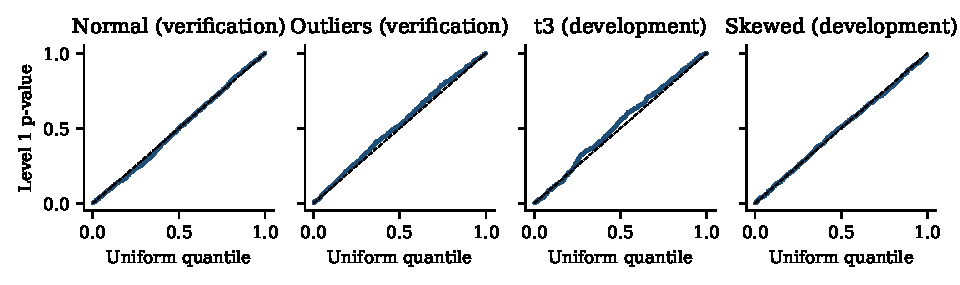
\includegraphics[width=\textwidth]{figures/fig_calibration.pdf}
\caption{Level 1 $p$-values under the null hypothesis against uniform quantiles, for four noise distributions (two verification and two development runs). The dashed line is the identity.}
\label{fig:calibration}
\end{figure}

\subsection{Across data sets, no $\Hone$ statistic separated the matched patterns}\label{sec:res-matched}
In the matched experiment, \nCentresOne{} of the \decOneN{} data sets at size 1 had one cycle centre, \nCentresTwo{} had two and \nCentresThree{} had three, with a median of \decOneChanged{} changed genes. Every directional statistic responded to the change, but by the pre-declared criterion no $\Hone$ statistic separated the cycle arm from the module arm: the AUC of $A_i$, its rank variant and $Z_i$ lay between 0.50 and \aucZTwo{} at both effect sizes (Table~\ref{tab:matched}). Signed Moran's $I$ (B2) separated the arms more strongly, in the opposite direction: its AUC was \aucBtwoOne{} and \aucBtwoTwo{}, an oriented AUC of \aucOrBtwoOne{} and \aucOrBtwoTwo{}, because in the module arm the centre changes together with its neighbours. Under the plan's rule, $\Hone$ therefore did not add information in this experiment. The variation between data sets, which differ in subnetwork and in the number of centres, was much larger than the difference between the arms.

The sign of $A_i$ is informative. A cycle of increased genes around an unchanged centre might be expected to raise $\Lup_i$ and make $A_i$ positive. Instead $A_i$ was strongly negative in both arms (mean $t=\tcycATwo$ in the cycle arm and $\tmodATwo$ in the module arm at size 2). We propose the following mechanism, which we have not verified at the level of individual intervals. In the lower-change filtration a block of increased genes enters last; the unchanged genes around it enter earlier and can form cycles that the block's genes fill when they enter, each with a lifetime close to the size of the change. Such cycles add to $\Ldown_i$ whether or not the block surrounds an unchanged gene, and they can be numerous. On an interaction network with many triangles, raw directional $\Hone$ persistence would then largely reflect where blocks of change sit, much like the $\Hzero$ asymmetry (B4, mean $t=\tcycBfourTwo$ and $\tmodBfourTwo$) and the component contrast (B3).

\begin{table}[t]
\centering\small
\caption{Matched cycle--module experiment, verification seeds (\decOneN{} data sets per size). Paired: share of data sets in which the statistic was larger in the cycle arm than in the module arm built from the same noise on the same subnetwork, with exact 95\% confidence intervals; there were \pairTies{} ties. $\Delta t$: mean paired difference $t_{\mathrm{cycle}}-t_{\mathrm{module}}$. AUC: $P(t_{\mathrm{cycle}}>t_{\mathrm{module}})$ over all pairs of data sets, ties counted one half; values below 0.5 mean the statistic is larger in the module arm. Size: change in units of the noise standard deviation.}
\label{tab:matched}
{\footnotesize\setlength{\tabcolsep}{4pt}\begin{tabular}{lrrrrrr}
\toprule
 & \multicolumn{3}{c}{Size 1} & \multicolumn{3}{c}{Size 2} \\
\cmidrule(lr){2-4}\cmidrule(lr){5-7}
Statistic & Paired (\%) & 95\% CI & AUC & Paired (\%) & 95\% CI & AUC \\
\midrule
$A_i$ (H1 asymmetry) & 61 & 54--68 & 0.51 & 72 & 65--78 & 0.52 \\
$A_i$, rank variant & 60 & 52--66 & 0.50 & 75 & 68--81 & 0.53 \\
$Z_i$ (network-adjusted) & 70 & 63--76 & 0.52 & 80 & 73--85 & 0.54 \\
B1 signed burden & 52 & 45--60 & 0.50 & 50 & 43--58 & 0.50 \\
B2 signed Moran's $I$ & 2 & 1--5 & 0.40 & 0 & 0--2 & 0.34 \\
B3 component size & 60 & 53--67 & 0.52 & 60 & 53--67 & 0.52 \\
B4 $H_0$ asymmetry & 44 & 37--51 & 0.47 & 44 & 37--51 & 0.47 \\
B9 local-extremum depth & 56 & 49--63 & 0.53 & 56 & 48--63 & 0.53 \\
\bottomrule
\end{tabular}
}
\end{table}

\subsection{Within matched pairs, the $\Hone$ statistics responded to the exchange}\label{sec:res-signal}
Holding the network and the noise fixed (Figure~\ref{fig:matched}), the $\Hone$ statistics were larger in the cycle arm than in its matched module arm more often than not, and more often at the larger effect size: $A_i$ in \pairAOne\% and \pairATwo\% of data sets at sizes 1 and 2, its rank variant in \pairArankOne\% and \pairArankTwo\%, and the network-adjusted $Z_i$ in \pairZOne\% (95\% CI \pairZOneci\%) and \pairZTwo\% (\pairZTwoci\%). At size 2 the mean paired difference of $Z_i$ was $\Delta t=\dtZTwo$ (95\% interval \dtciZTwo), and that of $A_i$ was \dtATwo. The topology-free statistics responded too, though less consistently: the local-extremum depth B9 was larger in the cycle arm in \pairBnineOne\% and \pairBnineTwo\% of data sets ($\Delta t=\dtBnineTwo$ at size 2), the component contrast B3 in \pairBthreeOne\% and \pairBthreeTwo\% ($\Delta t=\dtBthreeTwo$), and the $\Hzero$ asymmetry B4 in \pairBfourOne\% and \pairBfourTwo\% ($\Delta t=\dtBfourTwo$). The burden B1, which counts the same number of changed genes in both arms, behaved as a negative control (\pairBoneOne\% and \pairBoneTwo\%). Signed Moran's $I$ responded most strongly of all, in the opposite direction: B2 was larger in the cycle arm in only \pairBtwoOne\% and \pairBtwoTwo\% of data sets ($\Delta t=\dtBtwoTwo$ at size 2). The development runs, on different seeds, gave the same pattern ($Z_i$ in \devpairZOne\% and \devpairZTwo\%; Supplementary Table~\ref{tab:matcheddev}).

Paired wins and AUC are compatible. At size 2, $Z_i$ moved in the direction of the cycle arm in \pairZTwo\% of matched pairs, but by much less than its variation between networks, so it ordered data sets from different networks little better than chance. Because the exchange of centre and neighbour also changes the degrees, clustering and local autocorrelation of the changed genes, these paired results show that the $\Hone$ statistics are sensitive to this intervention; they do not show that the response is due to the hole, and they do not show that $\Hone$ carries information beyond the baselines jointly, which we have not tested.

\begin{figure}[t]
\centering
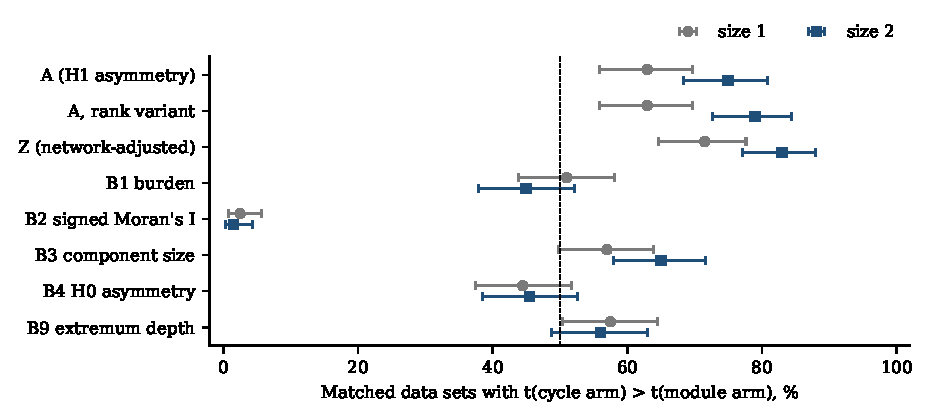
\includegraphics[width=\textwidth]{figures/fig_matched.pdf}
\caption{Matched cycle--module experiment. For each statistic, the share of matched data sets in which the statistic was larger in the cycle arm than in the module arm, with exact 95\% confidence intervals, at change sizes 1 (circles) and 2 (squares). There were no ties, so the dashed line at 50\% is the value expected if the exchange made no difference to the statistic.}
\label{fig:matched}
\end{figure}

\subsection{The network-adjusted reference did not absorb strong change at hubs}\label{sec:res-hub}
When only the genes in the top 5\% of degree changed, the raw asymmetry rejected $H_{\mathrm{sym}}$ in \hubA\% of \hubN{} data sets, as it should, since the change is real. The Level~2 test of $Z_i$ rejected in \hubZ\% of data sets (95\% CI \hubZci\%), and \hubZneg{} of the \hubZk{} rejections had a negative statistic. This is not a type~I error under $H_{\mathrm{sym}}$; it shows that the relabelling reference does not absorb this structured alternative, so that $Z_i$ would attribute it to arrangement. Two explanations are possible and we have not separated them. First, high-degree genes are interconnected in the graph used here: in the full STRING graph at score $\ge700$, the \hubHubN{} genes of the top 5\% of degree (degree $\ge\hubHubMinDeg$) share \hubHubObs{} edges, against a mean of \hubHubRew{} in \hubHubReps{} degree-preserving rewirings (ratio \hubHubRatio), and the degree assortativity is \degAssort. Relabelling within strata moves each hub's change to another gene of similar degree, but the genes that receive the changes are usually not adjacent, so the reference loses the adjacency among the changed hubs. This differs from the networks studied by \citet{maslov2002}, in which links between hubs were suppressed, and from the protein interaction network examined by \citet{colizza2006}, which showed no rich-club ordering; STRING includes members of protein complexes, which are densely linked. Second, the strata are coarse: the top 5\% of degree lies within the top decile, so relabelling within that decile moves changes to genes of lower degree even before adjacency is considered. A reference that preserves the adjacency among the changed genes would address the first explanation, and finer degree strata the second.

\subsection{Application to TCGA-BRCA}\label{sec:res-tcga}
The frozen analysis (Git tag \texttt{plan-v1.0}) was run on the \tcgaN{} patients. One technical amendment was made after the freeze and before any result was computed: arrays passed to GUDHI are copied, because GUDHI on Windows rejects the read-only memory-mapped arrays that the parallel back end uses for large inputs; it changes no value and is recorded in the file of amendments in \texttt{docs/provenance}. Table~\ref{tab:tcga} gives the patient-level results.

\paragraph{Paired asymmetry (Level 1).} The primary test rejected $H_{\mathrm{sym}}$ in both layers: RNA with $t=\tARna$ ($p_{\mathrm{Holm}}\pARna$; $A_i>0$ in \AposRna{} of \tcgaN{} patients) and methylation with $t=\tAMeth$ ($p_{\mathrm{Holm}}\pAMeth$; $A_i>0$ in only \AposMeth). The two results differ in robustness (Table~\ref{tab:tcgasens}). The RNA result changed sign with the rank variant ($t=\tArankRna$), the standardised change and both alternative network thresholds, and was not significant after composition adjustment or in pairs whose two specimens share a plate; it also weakened under added measurement noise (median $t$ \noiseTenRna, \noiseTwentyFiveRna{} and \noiseFiftyRna{} at 10\%, 25\% and 50\% of each gene's SD). The RNA Level~1 rejection is therefore not supported by the pre-specified sensitivity analyses. The methylation asymmetry was negative on the observed $M$-value scale in every pre-specified analysis except the rank variant ($t=\tArankMeth$), so it depends on the magnitudes of the changes and not only on their order; it was almost unchanged by noise (median $t$ \noiseFiftyMeth{} at 50\%). Its direction is the one that the proposed mechanism of Section~\ref{sec:res-matched} associates with connected blocks of increased change, and the non-topological baselines point the same way: more promoters were hypermethylated than hypomethylated among the analysed genes (B1, $t=\tBoneMeth$), and the hypermethylated genes formed larger components (B3, $t=\tBthreeMeth$) with stronger graph autocorrelation (B2, $t=\tBtwoMeth$). These statements concern the \methGenes{} analysed promoter-associated genes, not genome-wide methylation. Moran's $I$ of the change was positive on average in both layers. The two layers' asymmetries were weakly negatively correlated across patients (Spearman $\rho=\crossRho$, 95\% CI \crossRhoCI; exploratory).

\begin{table}[t]
\centering\small
\caption{TCGA-BRCA, \tcgaN{} tumour--normal pairs: studentized mean $t$ over patients and sign-flip $p$-value with Holm over the two layers ($B=9{,}999$, so the smallest attainable $p$ is $10^{-4}$). Upper block: topological statistics; the composition-adjusted $Z_i$ is an exploratory analysis decided after the frozen results were seen. Lower block: baselines on the same patients and sign flips.}
\label{tab:tcga}
\begin{tabular}{lrrrr}
\toprule
 & \multicolumn{2}{c}{RNA} & \multicolumn{2}{c}{Methylation} \\
\cmidrule(lr){2-3}\cmidrule(lr){4-5}
Statistic & $t$ & $p_{\mathrm{Holm}}$ & $t$ & $p_{\mathrm{Holm}}$ \\
\midrule
$A_i$ ($H_1$ asymmetry), Level 1 & +2.16 & 0.032 & -9.74 & $<$0.001 \\
$A_i$, rank variant & -2.37 & 0.038 & +1.19 & 0.231 \\
$Z_i$ (network-adjusted), Level 2 & +8.14 & $<$0.001 & +1.56 & 0.125 \\
$Z_i$, composition-adjusted (exploratory) & +6.38 & $<$0.001 & +1.97 & 0.057 \\
\midrule
B1 signed burden & +0.77 & 0.440 & +8.02 & $<$0.001 \\
B2 signed Moran's $I$ & -0.37 & 0.704 & +6.39 & $<$0.001 \\
B3 component size & +1.92 & 0.057 & +6.56 & $<$0.001 \\
B4 $H_0$ asymmetry & -15.20 & $<$0.001 & +10.27 & $<$0.001 \\
B9 local-extremum depth & +14.74 & $<$0.001 & -10.72 & $<$0.001 \\
B8 specimen-level $H_1$ & +6.83 & $<$0.001 & +5.92 & $<$0.001 \\
\bottomrule
\end{tabular}

\end{table}

\paragraph{Network-adjusted asymmetry (Level 2).} The reference used $R=199$ relabellings per patient within \methStrata{} (methylation) and \rnaStrata{} (RNA) non-empty strata; the reference spread fell below the floor in \atFloorRna{} (RNA) and \atFloorMeth{} (methylation) patients. For methylation the network-adjusted score was not significant ($t=\tZMeth$, $p_{\mathrm{Holm}}\pZMeth$; mean $Z_i=\ZmeanMeth$, 95\% CI \ZciMeth): the data do not show a systematic departure of the methylation asymmetry from the specified relabelling reference. This does not show that the arrangement of methylation changes is random on the network; B2 and B3 indicate that hypermethylated promoters are clustered. For RNA the network-adjusted score was consistent across patients but modest in each: $t=\tZRna$ ($p_{\mathrm{Holm}}\pZRna$), $Z_i>0$ in \ZposRna{} of \tcgaN, mean $Z_i=\ZmeanRna$ (95\% CI \ZciRna), median \ZmedRna, and $|Z_i|\le\ZmaxRna$ in every patient (Figure~\ref{fig:tcgaz}). The large $t$ reflects the consistency of a small departure across patients, not a large departure in any one. On the scale of the asymmetry, the observed $A_i$ averaged \AmeanRna{} against a reference mean of \AmuRna{} for the same changes relabelled within strata; the difference $A_i-\mu_i$ had median \AmuMedRna{} (interquartile range \AmuIQRRna). The raw RNA asymmetry was thus small and unstable, while its departure from the reference was consistent. Because composition was adjusted only at Level~1 in the plan, and composition removed the RNA Level~1 effect, we added one exploratory analysis after seeing these results: the same Level~2 test after regressing the stromal and immune proxies out of the change. The RNA score remained ($t=\tZcompRna$, $p_{\mathrm{Holm}}\pZcompRna$; $Z_i>0$ in \ZcompposRna{} patients); the mean $Z_i$ fell by \ZcompdropRna\%, and the adjusted and unadjusted scores were highly correlated across patients ($r=\ZcompcorrRna$). The methylation score stayed non-significant ($t=\tZcompMeth$). The simulations limit how the RNA result can be read: $Z_i$ is not specific to holes, and it responds to changed genes that are adjacent to one another (Section~\ref{sec:res-hub}). By the mechanism proposed in Section~\ref{sec:res-matched}, a positive $Z_i$ is consistent with connected groups of \emph{decreased} genes that fill cycles of the higher-change filtration, as well as with cycles of increased genes. Robustness analyses with a single relabelling applied to all patients, and with degree-preserving rewiring (which removed about 95\% of the triangles, \obsTriRna{} to a median of \rewireTriRna), showed that the Level~1 statistic depends strongly on the network's local structure (median $t$ \rewireTRna{} and \rewireTMeth{} on rewired networks; descriptive).

\begin{figure}[t]
\centering
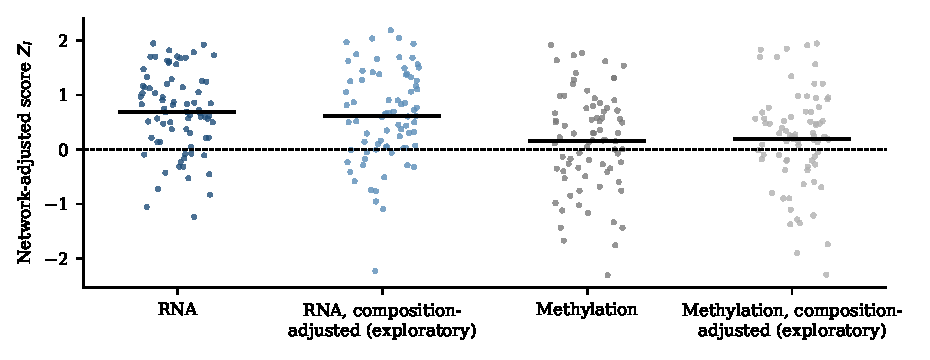
\includegraphics[width=\textwidth]{figures/fig_tcga_z.pdf}
\caption{Network-adjusted scores $Z_i$ of the \tcgaN{} patients, before and after the exploratory composition adjustment. Bars mark the means; the dashed line marks zero.}
\label{fig:tcgaz}
\end{figure}

\begin{table}[t]
\centering\small
\caption{Pre-specified sensitivity analyses of the Level~1 asymmetry $A_i$. The alternative STRING thresholds use the genes of the primary network (Section~\ref{sec:cohort}). Same-plate pairs: one layer each, unadjusted $p$.}
\label{tab:tcgasens}
\begin{tabular}{lrrrr}
\toprule
 & \multicolumn{2}{c}{RNA} & \multicolumn{2}{c}{Methylation} \\
\cmidrule(lr){2-3}\cmidrule(lr){4-5}
Analysis & $t$ & $p_{\mathrm{Holm}}$ & $t$ & $p_{\mathrm{Holm}}$ \\
\midrule
Primary (plain change, STRING $\ge$700) & +2.16 & 0.032 & -9.74 & $<$0.001 \\
Rank variant & -2.37 & 0.038 & +1.19 & 0.231 \\
Standardised change & -3.50 & 0.001 & -7.26 & $<$0.001 \\
STRING $\ge$400 & -6.50 & $<$0.001 & -13.95 & $<$0.001 \\
STRING $\ge$900 & -5.12 & $<$0.001 & -11.17 & $<$0.001 \\
Composition-adjusted & +1.56 & 0.119 & -8.77 & $<$0.001 \\
Same-plate pairs (60 / 45) & +1.45 & 0.157 & -9.22 & $<$0.001 \\
\bottomrule
\end{tabular}

\end{table}

\paragraph{Placebo.} In \placeboN{} data sets of pseudo-pairs formed from the tumours of different patients, Level~1 rejected in \placeboRna\% (RNA) and \placeboMeth\% (methylation) of data sets, in line with the nominal 5\% for this number of data sets.

\paragraph{Genes (Level 3).} Of the \geneFamily{} layer--gene pairs in the family (\audFamRna{} RNA, \audFamMeth{} methylation), \geneSig{} were significant after Holm (\geneSigRna{} RNA, \geneSigMeth{} methylation; smallest attainable $p=\minP$). These are layer--gene associations; they involve \geneUnique{} distinct genes. Each was stable by the pre-specified rule: in at least 50\% of 100 random half-samples of patients, its sign-flip test (999 flips) gave $p\le0.05$ with the same sign; all \geneStable{} met this rule. Under the reversed tie rule, \geneTiePct\% of the \geneSig{} kept the sign of their score; sign agreement does not show that representative membership is stable. The strongest RNA participants (Table~\ref{tab:tcgagenes}) are proliferation genes on cycles of the higher-change filtration (CCNA2, AURKA, PCNA, CDK1, CDC45, EZH2) together with FN1 and TGFB1, and vascular, stromal and adipose-associated genes on cycles of the lower-change filtration (VWF, ELN, DCN, CAV1, NID1, LRP1); the strongest methylation participants are dominated by immune genes. These match the known contrast between breast tumours and adjacent normal tissue \citep{tcga2012} and are consistent with differences in proliferation and in cell composition.

Table~\ref{tab:geneaudit} compares the topological participants with the single-gene test B6 and the smoothed test B7. As run, B6 and B7 used Holm over all genes of the layer network (\audNetRna{} RNA and \audNetMeth{} methylation), a larger family than the topology family; we also recomputed Holm for B6 over the topology family alone, which is the comparison on equal terms. On equal terms, \audNotBsixfRna{} of the \audTopoRna{} RNA participants (\audNotBsixfPctRna\%) and \audNotBsixfMeth{} of the \audTopoMeth{} methylation participants (\audNotBsixfPctMeth\%) were not significant as single genes; \audNotBothRna{} (\audNotBothPctRna\%) and \audNotBothMeth{} (\audNotBothPctMeth\%) were significant by neither B6 nor B7. A gene that is not significant after Holm can still have a substantial but variable change. In RNA, for example, DTNB was essentially unchanged (single-gene $t=\sgDtnb$), whereas SNTB1 ($t=\sgSntb$) and DAG1 ($t=\sgDag$) changed but did not reach Holm significance; all three belong to the dystrophin-associated protein complex. In methylation, the promoter of TNFRSF13C (the BAFF receptor) was unchanged as a single gene ($t=\sgBaffr$) but a strong participant, as was its ligand TNFSF13B ($t=\sgBaff$ as a single gene); we have not checked whether the two genes lie on the same cycle representatives, so their known interaction does not show co-attribution. Under the pre-declared outcome (below) these genes are candidates for follow-up, not gene-specific findings.

\begin{table}[t]
\centering\small
\caption{Topological participants compared with the single-gene test (B6) and the neighbourhood-smoothed test (B7), counted from the result files. Holm-significant at 0.05 throughout. ``Family Holm'': Holm recomputed over the topology family only, so that B6 and the topology test are adjusted over the same genes.}
\label{tab:geneaudit}
\begin{tabular}{lrr}
\toprule
 & RNA & Methylation \\
\midrule
Genes in the layer network (B6 and B7 were tested on all) & 7,624 & 8,438 \\
Topology family (non-zero score in $\ge$10 patients) & 2,595 & 2,823 \\
Topology: Holm-significant in its family & 833 & 446 \\
B6 single gene: Holm over network genes & 3,217 & 1,905 \\
B6 single gene: Holm over the topology family & 1,251 & 643 \\
B7 smoothed: Holm over network genes & 3,025 & 2,762 \\
\midrule
Topology, not B6 (Holm over network genes) & 333 & 221 \\
Topology, not B6 (Holm over the topology family) & 300 & 209 \\
Topology, not B7 & 460 & 182 \\
Topology, neither B6 nor B7 & 201 & 97 \\
\bottomrule
\end{tabular}

\end{table}

\begin{table}[t]
\centering\small
\caption{The 15 Holm-significant topological participants with the largest $|t|$ per layer. Positive $t$: on cycles of the higher-change filtration (increased genes); negative: of the lower-change filtration. Single-gene: Holm-significant in the paired single-gene test B6 (Holm over the network genes).}
\label{tab:tcgagenes}
\begin{tabular}{lrc|lrc}
\toprule
\multicolumn{3}{c|}{RNA} & \multicolumn{3}{c}{Methylation} \\
Gene & $t$ & Single-gene & Gene & $t$ & Single-gene \\
\midrule
FN1 & +22.9 & yes & CX3CL1 & +17.1 & yes \\
VWF & -21.5 & yes & CD40 & +14.7 & yes \\
CCNA2 & +20.4 & yes & TNFSF8 & -14.1 & yes \\
TGFB1 & +18.8 & yes & BICD2 & -14.0 & no \\
DTNB & +17.1 & no & RAB6A & -14.0 & no \\
PARP1 & +16.5 & yes & BICDL1 & -13.8 & no \\
ELN & -16.3 & no & TNFSF13B & -13.6 & no \\
PCNA & +16.1 & yes & CXCL1 & +13.2 & yes \\
SNTB1 & +16.1 & no & TNFRSF13C & -13.0 & no \\
AURKA & +15.9 & yes & PTEN & -12.8 & no \\
ATP6V0B & +15.7 & yes & CD80 & -12.3 & yes \\
CLSPN & +15.1 & yes & PSIP1 & -11.8 & no \\
RPA1 & -14.9 & no & ESR1 & -11.8 & yes \\
EGFR & -14.8 & yes & FGF2 & +11.4 & yes \\
TGFBR2 & -14.6 & yes & ITGB3 & +11.2 & yes \\
\bottomrule
\end{tabular}

\end{table}

\paragraph{Pre-declared outcome.} The plan defines the outcomes by whether Levels~1 and~2 are supported, without saying whether a primary rejection that the sensitivity analyses do not support counts as support. For methylation the answer does not matter: Level~1 rejected and kept its direction in every sensitivity analysis but the rank variant, and Level~2 did not reject, which is outcome C (directional asymmetry without demonstrated network specificity). For RNA it does. Reading ``supported'' as ``rejected in the primary test'', Levels~1 and~2 both rejected and the genes are unconfirmed, which is outcome B (a patient-level result without gene-specific claims). Reading it as ``rejected and robust'', Level~1 is not supported, which is outcome D for the paired asymmetry, with the Level~2 result reported as a secondary finding. We report both readings. Under either, the plan allows no gene-specific claims.
